\documentclass[11pt,a4paper]{article}

\usepackage[T1]{fontenc}
\usepackage[utf8]{inputenc}
\usepackage{lmodern}
\usepackage{microtype}
\usepackage[a4paper,margin=25mm,headheight=15pt]{geometry}
\usepackage{amsmath,amssymb,bm}
\usepackage{booktabs,longtable,array,tabularx}
\usepackage{graphicx}
\usepackage{float}
\usepackage{xcolor}
\usepackage{enumitem}
\usepackage{fancyhdr}
\usepackage{titlesec}
\usepackage{listings}
\usepackage{caption}
\usepackage{hyperref}
\usepackage{xurl}

\definecolor{ink}{HTML}{17191C}
\definecolor{muted}{HTML}{5D646C}
\definecolor{amber}{HTML}{A85D00}
\definecolor{cyan}{HTML}{126878}
\definecolor{panel}{HTML}{F4F1EA}
\definecolor{codebg}{HTML}{F1F3F4}
\hypersetup{
  colorlinks=true,
  linkcolor=cyan,
  citecolor=amber,
  urlcolor=cyan,
  pdftitle={Betelgeuse Observatory: Scientific and Engineering Report},
  pdfauthor={Biswajit Jana}
}
\pagestyle{fancy}
\fancyhf{}
\lhead{Betelgeuse Observatory}
\rhead{Biswajit Jana}
\cfoot{\thepage}
\setlength{\parindent}{0pt}
\setlength{\parskip}{0.65em}
\setlist{nosep,leftmargin=1.5em}
\titleformat{\section}{\Large\bfseries\color{ink}}{\thesection}{0.6em}{}
\titleformat{\subsection}{\large\bfseries\color{ink}}{\thesubsection}{0.6em}{}
\captionsetup{font=small,labelfont=bf}
\lstset{
  basicstyle=\ttfamily\small,
  backgroundcolor=\color{codebg},
  frame=single,
  rulecolor=\color{codebg},
  breaklines=true,
  columns=fullflexible,
  showstringspaces=false
}
\newcommand{\evidence}[1]{\textcolor{cyan}{\textbf{#1}}}
\newcommand{\caveat}[1]{\textcolor{amber}{\textbf{#1}}}
\newcommand{\Rsun}{R_{\odot}}
\newcommand{\Msun}{M_{\odot}}

\title{\vspace{-1.2cm}\textbf{Betelgeuse Observatory}\\[0.35em]
\large A Causal, Quantitative, and Physics-Coupled Research Platform}
\author{\textbf{Biswajit Jana}\\Research author and project lead}
\date{31 August 2026}

\begin{document}
\maketitle

\begin{abstract}
I designed and implemented Betelgeuse Observatory as a reproducible research platform for a question that is simple to state but easy to mishandle: what can present observations establish about Betelgeuse, and what can they support about the time at which a future core-collapse signal may reach Earth? The project combines a light-cone derivation, published ALMA continuum measurements, parametric contour diagnostics, a spectral and image-sequence workbench, explicitly separated stellar-evolution scenarios, and an interactive three-dimensional atmosphere driven by a reduced gas-flow solver. My central result is epistemic as much as numerical. No received observation establishes core collapse. Under my preferred interpretation of the approximately 400--416 day signal as the radial fundamental mode and the approximately 2170 day long secondary period as companion-related, a representative remaining-time point is $2\times10^5$ years, mapping to approximately 202,026 CE at Earth. This is a declared scenario point, not a fitted date or confidence interval. A contested late-carbon-burning interpretation gives a much shorter illustrative arrival interval of 2056--2326 CE, but depends on a disputed pulsation-mode assignment and radius. This report documents the complete scientific rationale, equations, implementation, verification, limitations, and reproduction path.
\end{abstract}

\vspace{0.5em}
\begin{center}
\fcolorbox{cyan}{panel}{\parbox{0.91\textwidth}{
\textbf{Scientific verdict.} As of 31 August 2026, the defensible statement is that Betelgeuse has a resolved, asymmetric, time-variable atmosphere. The data do not show a received supernova signal and do not permit observation beyond Earth's past light cone. Atmospheric structure is evidence about the atmosphere; it is not by itself a calibrated probability of imminent core collapse.
}}
\end{center}

\tableofcontents
\clearpage

\section{Research question and design philosophy}

I began by dividing the broad question ``Has Betelgeuse already exploded?'' into three distinct questions:

\begin{enumerate}
  \item What physical state of the star is contained in the radiation reaching Earth now?
  \item Given that observed state, what remaining lifetime is supported by each stellar-evolution model family?
  \item If collapse occurs after a remaining interval $\Delta t$ at the star, when does its signal arrive at Earth?
\end{enumerate}

This decomposition prevents a common category error: subtracting the light-travel time twice. It also forces each website panel to state whether it shows a measured quantity, a deterministic calculation, a simulation, a model-dependent inference, or a speculative scenario. I used those five claim classes throughout the interface. The labels are semantic, visible, and text based; colour is only a secondary cue.

My engineering decisions followed the same principle. Small, auditable functions perform the causal, angular, continuum, and forecast calculations. Published numbers are kept in a compact redistributable table. Large observatory products are represented by provenance records rather than committed files. The interactive visualizations explain the physics without pretending that a rendered image is calibrated data.

\section{Evidence boundary and provenance}

The latest evidence used by the platform is organized by observation epoch, publication date, instrument, frequency, spatial response, and product status. This matters because a preprint published in 2026 can analyse photons recorded in 2023. ``Latest paper'' and ``latest state observed'' are not equivalent phrases.

The core datasets are summarized in Table~\ref{tab:data}. Exact access notes and local target paths are recorded in \texttt{data/manifest.yaml}. Raw FITS, measurement sets, and other large scientific products are excluded from version control.

\begin{table}[H]
\centering
\caption{Primary observational inputs and their role in the project.}
\label{tab:data}
\small
\begin{tabularx}{\textwidth}{@{}>{\raggedright\arraybackslash}p{0.23\textwidth}>{\raggedright\arraybackslash}p{0.18\textwidth}>{\raggedright\arraybackslash}X>{\raggedright\arraybackslash}p{0.20\textwidth}@{}}
\toprule
Dataset & Epoch & Scientific role & Repository status \\
\midrule
ALMA 2022.A.00026.S & August 2023 & Bands 6, 7, and 8 continuum and molecular structure & Published values and attributed preview \\
ALMA 2015.1.00206.S & 9 November 2015 & Beam-aware temporal comparison target & Provenance record \\
ESO 114.28H9 & 6 December 2024 & SPHERE-ZIMPOL companion candidate & Official archive reference \\
Herschel / Lloyd & 1836--1840 & Earliest reconstructed visual estimates & 27 attributed values \\
AAVSO AID & 1893--2026 & Long-baseline visual and Johnson V photometry & 51,460 screened detections \\
MAST/HST & Product dependent & Ultraviolet chromosphere and wind spectra & Retrieval contract \\
\bottomrule
\end{tabularx}
\end{table}

The ALMA editorial image in Figure~\ref{fig:alma} is included for orientation and attribution. I do not measure pixels from it. Publication-grade analysis must start from calibrated archive products, preserve the restoring beam and units, and record the reduction procedure.

\begin{figure}[H]
\centering
\IfFileExists{public/observations/alma-band8-2023.png}{
  
\includegraphics[width=0.78\textwidth]{public/observations/alma-band8-2023.png}
}{
  \IfFileExists{../public/observations/alma-band8-2023.png}{
    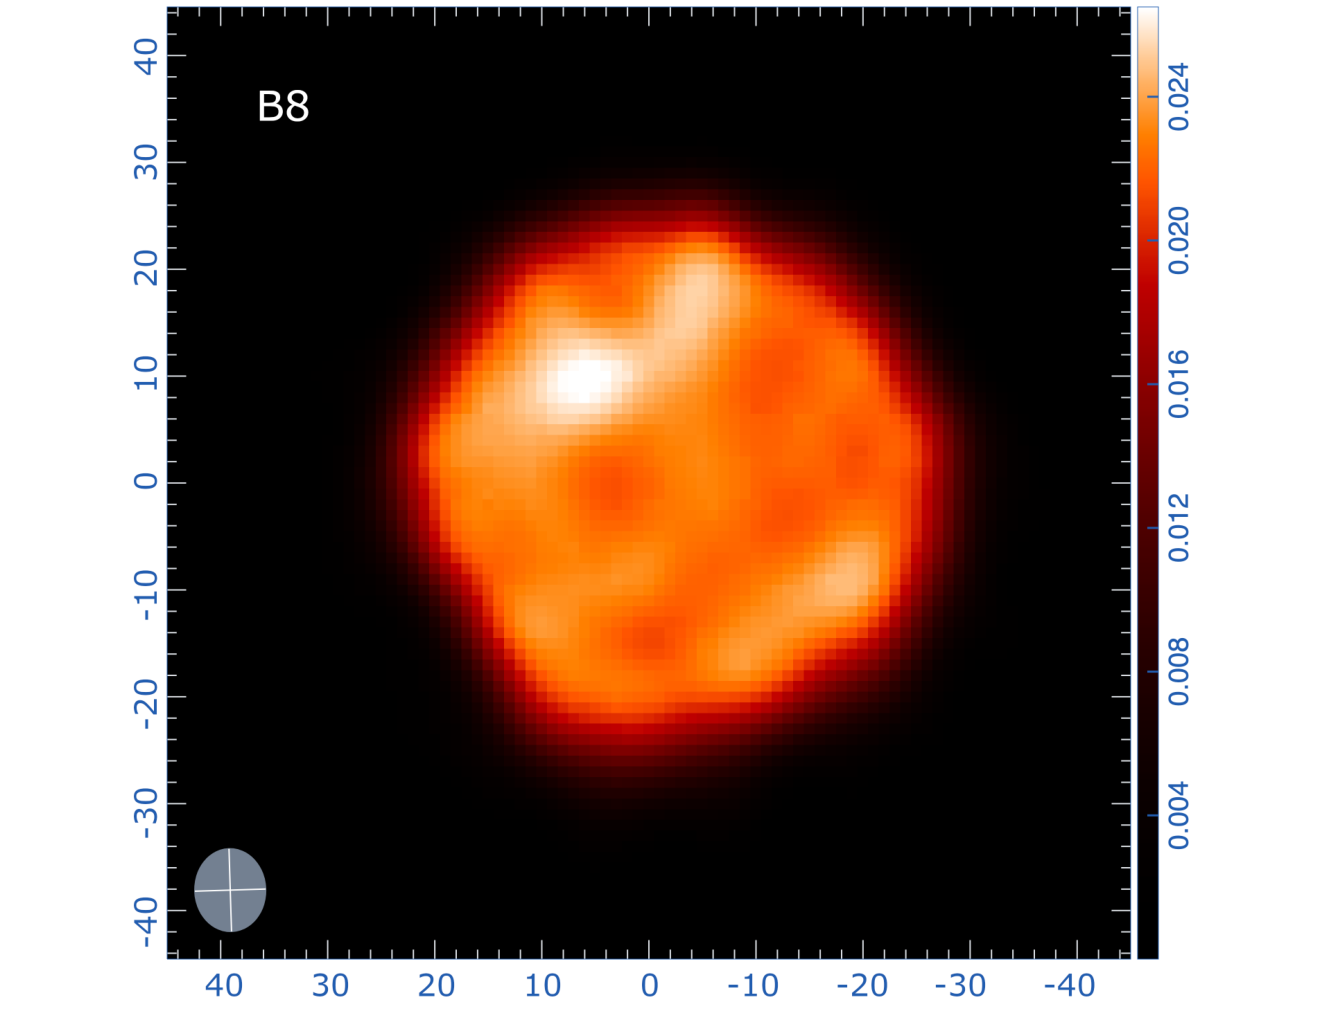
\includegraphics[width=0.78\textwidth]{../public/observations/alma-band8-2023.png}
  }{\fbox{\parbox{0.75\textwidth}{ALMA Band 8 preview is available in the repository at \texttt{public/observations/alma-band8-2023.png}.}}}
}
\caption{ALMA Band 8 editorial preview of Betelgeuse, observed on 1 August 2023. Source: Dent et al. (2026), programme 2022.A.00026.S, CC BY 4.0. This rendered image is contextual, not a quantitative analysis input.}
\label{fig:alma}
\end{figure}

\subsection{Historical brightness record}

I treat the long brightness history as photometry rather than as an image
sequence. The earliest layer consists of 27 visual magnitudes reconstructed by
Lloyd from William Herschel's 1836--1840 comparison-star sequences
\cite{lloyd2020}. The machine-readable layer comes from the AAVSO International
Database, target AUID \texttt{000-BBK-383} \cite{aavso2026}. My reproducible
query returned 51,546 rows spanning 10 December 1893 to 30 August 2026. I
excluded 55 upper-limit rows and 31 values outside the deliberately broad
$-0.5\leq m\leq3.0$ target-specific plausibility screen, leaving 48,378 visual
and 3,082 Johnson V detections.

I never merge the two AAVSO passbands. For each passband and time bin $k$, the
displayed central value and descriptive scatter are
\begin{equation}
  \widetilde m_k=\operatorname{median}_{i\in k}(m_i),\qquad
  \operatorname{IQR}_k=Q_{3,k}-Q_{1,k}.
\end{equation}
The full 1836--2026 view uses 90-day bins and the 2010--2026 detail uses 30-day
bins. Empty bins remain empty, so no line is drawn across a sufficiently long
gap. The optional relative-flux view applies the exact magnitude relation
\begin{equation}
  \frac{F}{F_0}=10^{-0.4(m-m_0)},\qquad m_0=0.5,
\end{equation}
and is a change of scale rather than a forecast. The committed derived CSV
contains medians, quartiles, median absolute deviations, bin populations,
Julian dates, and decimal years. The row-level AAVSO export remains in the
gitignored raw-data area and can be regenerated with
\texttt{science/ingestion/aavso\_history.py}.

This distinction is central to the website design. Nineteenth-century visual
estimates contain no resolved surface information, and most of the AAVSO
record is unresolved photometry. Rendering those numbers as synthetic stellar
images would manufacture morphology that was never observed. The brightness
record is therefore plotted; only modern, registered, matched-resolution image
products belong in the blink comparator.

\section{Causality and light-travel time}

Let $t_{\mathrm{receive}}$ be the time at which Earth receives a photon emitted by Betelgeuse at $t_{\mathrm{emit}}$. For distance $D$,
\begin{equation}
t_{\mathrm{emit}} = t_{\mathrm{receive}} - \frac{D}{c}.
\end{equation}
If the star has a remaining lifetime $\Delta t$ measured from that emitted state, then collapse occurs at
\begin{equation}
t_{\mathrm{collapse}} = t_{\mathrm{emit}} + \Delta t.
\end{equation}
The collapse signal then traverses the same distance:
\begin{align}
t_{\mathrm{arrival}}
  &= t_{\mathrm{collapse}} + \frac{D}{c} \\
  &= t_{\mathrm{receive}} - \frac{D}{c} + \Delta t + \frac{D}{c} \\
  &= \boxed{t_{\mathrm{receive}} + \Delta t}.
\end{align}

The cancellation is exact within the assumed stationary geometry. Distance uncertainty changes which historical stellar epoch is currently visible; it does not change the waiting time implied by a remaining-lifetime estimate conditioned on that visible state. The interactive causality laboratory samples the asymmetric distance estimate $D=172^{+13}_{-11}$ pc with a two-piece normal distribution and displays both the reconstructed emission epoch and the invariant arrival relation.

For a one-way distance expressed in parsecs, the approximate look-back time is
\begin{equation}
\tau_{\mathrm{lt}}\,[\mathrm{yr}] = 3.26156\,D\,[\mathrm{pc}],
\end{equation}
so the central value corresponds to roughly 561 light-years. This number is scientifically relevant to the epoch being observed, but it is not a correction to add again to $\Delta t$.

\section{Angular size and physical scale}

The small-angle relation connects angular diameter $\theta$, distance $D$, and physical radius $R$:
\begin{equation}
R = \frac{D\theta}{2}, \qquad \theta\ \text{in radians}.
\end{equation}
Using milliarcseconds and parsecs,
\begin{equation}
\frac{R}{\Rsun} = \frac{D_{\mathrm{pc}}\,\theta_{\mathrm{mas}}}{2}
\frac{1\ \mathrm{AU}}{\Rsun}.
\end{equation}
This conversion is implemented and unit tested because radius is central to the disagreement between the short- and long-horizon stellar models. A mode identification that demands a radius inconsistent with interferometric or radio angular sizes carries a direct observational tension.

The same geometry is used for the conditional supernova shell. If ejecta expand ballistically with speed $v_{\mathrm{ej}}$ for time $\Delta t$, then
\begin{equation}
R_{\mathrm{ej}}=v_{\mathrm{ej}}\Delta t,\qquad
\theta_{\mathrm{ej}}\simeq \frac{2R_{\mathrm{ej}}}{D}.
\end{equation}
The website keeps this physical angular scale separate from the compressed visual scale required to keep an expanding shell on screen.

\section{ALMA continuum fit}

The small continuum sample reproduces a transparent three-point power-law check. The measurements are given in Table~\ref{tab:alma}. These are integrated continuum quantities; they do not replace matched-beam spatial analysis.

\begin{table}[H]
\centering
\caption{Published 2023 ALMA continuum values used by the quantitative panels.}
\label{tab:alma}
\begin{tabular}{@{}lrrrr@{}}
\toprule
Band & $\nu$ (GHz) & $S_\nu$ (Jy) & $\sigma_S$ (Jy) & Diameter (mas) \\
\midrule
6 & 223.55 & 0.28 & 0.014 & 62.14 \\
7 & 337.99 & 0.51 & 0.040 & 57.74 \\
8 & 485.22 & 0.90 & 0.090 & 54.30 \\
\bottomrule
\end{tabular}
\end{table}

I fit
\begin{equation}
S_\nu=A\left(\frac{\nu}{\nu_0}\right)^\alpha
\end{equation}
by weighted least squares in log space. Define
\begin{equation}
x_i=\ln(\nu_i/\nu_0),\qquad y_i=\ln S_i,\qquad
\sigma_{y_i}\simeq \frac{\sigma_{S_i}}{S_i},
\end{equation}
and minimize
\begin{equation}
\chi^2(A,\alpha)=\sum_i\frac{[y_i-\ln A-\alpha x_i]^2}{\sigma_{y_i}^2}.
\end{equation}
With $\nu_0=337.99$ GHz, the implementation obtains
\begin{equation}
\alpha=1.494\pm0.133,\qquad A=0.518\ \mathrm{Jy}.
\end{equation}

This slope is calculated from three integrated values and should be interpreted at that level. The frequency-dependent angular diameter decreases from 62.14 mas in Band 6 to 54.30 mas in Band 8, consistent with different optical-depth surfaces. It is not evidence that the material sphere itself changes size between simultaneous frequencies.

The in-band workbench evaluates the same law only within the observed frequency range. For a candidate measurement $S_{\nu,*}$, it reports a standardized residual
\begin{equation}
z_* = \frac{S_{\nu,*}-\widehat{S}_{\nu,*}}
{\sqrt{\sigma_{\mathrm{meas},*}^{2}+\sigma_{\mathrm{model},*}^{2}}}.
\end{equation}
The interface warns that calibration covariance and intrinsic variability are incomplete in this demonstration; consequently $z_*$ is a triage statistic, not a discovery significance.

\section{Contour and radial diagnostics}

I added the contour laboratory to explain how a resolved continuum image is decomposed and tested. The principal field is
\begin{equation}
I_\nu^{\mathrm{model}}(x,y)=I_{\mathrm{disk}}(x,y)+I_{\mathrm{ext}}(x,y)
+\sum_k A_k\exp\left[-\frac{1}{2}r_k^2(x,y)\right],
\end{equation}
where each $r_k$ is an elliptical radius after rotation by a component position angle. For offsets $\Delta x$ and $\Delta y$,
\begin{align}
x' &= \Delta x\sin\phi + \Delta y\cos\phi,\\
y' &= \Delta x\cos\phi - \Delta y\sin\phi,\\
r^2 &= \frac{x'^2}{\sigma_{\rm maj}^2}+\frac{y'^2}{\sigma_{\rm min}^2},
\qquad \sigma_{\rm maj}=\frac{\mathrm{FWHM}_{\rm maj}}{2\sqrt{2\ln2}}.
\end{align}

The Band 8 reconstruction uses the published 54.30 mas disk diameter, axial ratio 0.98, and position angle 33 degrees. The northeast Gaussian is anchored at $(+10.1,+9.2)$ mas with 10.9 mas major-axis FWHM, axial ratio 0.86, and position angle 111 degrees. The northern compact component is anchored at $(-2.1,+17.7)$ mas. A southwest enhancement and belt term illustrate morphology that cannot be uniquely recovered from the rendered paper figure.

The displayed contour levels are 4, 8, 12, 16, 20, 22, 23, 24, 25, and 26 mJy beam$^{-1}$. A dashed 42 mas circle supplies the nominal optical scale, and a 7.7 by 6.6 mas ellipse supplies the Band 8 restoring-beam scale. Marching squares converts the sampled scalar field to line segments. For each grid cell, a four-bit case index identifies the intersections of an isovalue with the cell edges; linear interpolation locates the crossing.

The residual diagnostic is
\begin{equation}
\Delta I_\nu(x,y)=I_\nu(x,y)-I_{\nu,\mathrm{axi}}(x,y).
\end{equation}
Warm solid contours mark positive residuals and cool dashed contours mark negative residuals at absolute levels 2 and 4 mJy beam$^{-1}$. Their morphology is explicitly illustrative. A calibrated residual requires visibility-domain fitting, a noise covariance model, and a consistent beam.

For two matched-beam radial profiles, the spectral index is
\begin{equation}
\alpha(r)=\frac{\ln[I_8(r)/I_7(r)]}{\ln(\nu_8/\nu_7)}.
\end{equation}
Real maps must be registered, convolved to a common beam, masked by a stated signal-to-noise criterion, and propagated with both calibration and map uncertainty. The website's smooth profiles teach that calculation; they are not measured profiles.

\section{Spectral and image-sequence analysis}

The spectrum workbench is built around observables, not labels. A line with rest wavelength $\lambda_0$ has line-of-sight velocity
\begin{equation}
v_{\mathrm{los}}\simeq c\frac{\lambda-\lambda_0}{\lambda_0}
\end{equation}
in the non-relativistic limit. Equivalent width is
\begin{equation}
W_\lambda=\int\left(1-\frac{F_\lambda}{F_{\lambda,c}}\right)d\lambda,
\end{equation}
while asymmetry, width, velocity centroid, and multi-component structure test changes in atmospheric dynamics. These features are meaningful only when wavelength calibration, line-spread function, continuum placement, units, and uncertainties are retained.

For image epochs $I_t$, a quantitative difference requires registration and a common effective beam $B$:
\begin{equation}
\Delta I_t=(I_t\ast K_t)-(I_{t-1}\ast K_{t-1}),
\end{equation}
where $K_t$ maps each epoch to the chosen common beam. A standardized difference can then be formed as
\begin{equation}
Z_t(x,y)=\frac{\Delta I_t(x,y)}
{\sqrt{\sigma_t^2(x,y)+\sigma_{t-1}^2(x,y)}}.
\end{equation}

The browser comparator can blink as many as 5,000 local PNG, JPEG, or WebP frames. It is intentionally visual-only: local files are decoded in the browser, ordered, played, paused, scrubbed, and cleared without being uploaded. Quantitative differencing is refused unless calibrated, registered, beam-matched products are supplied. This separation lets the interface support rapid human inspection without assigning scientific confidence to display pixels.

The long-baseline photometric graph and the blink comparator are therefore
complementary rather than interchangeable: the first measures unresolved
brightness versus time, while the second inspects spatial morphology in modern
resolved products.

\section{Evolutionary scenarios and prediction}

The relevant pulsation scaling is
\begin{equation}
P_n=Q_n\sqrt{\frac{R^3}{GM}},
\end{equation}
where $Q_n$ depends on radial order and internal structure. Identifying a period as the fundamental mode therefore constrains the mean density and radius; mode assignments cannot be exchanged without changing the stellar model.

\subsection{Preferred long-horizon branch}

My preferred interpretation treats the approximately 400--416 day signal as the radial fundamental mode and the approximately 2170 day long secondary period as companion-related. This is compatible with an early core-helium-burning model family and a remaining lifetime of order hundreds of thousands of years. I select one representative point for a transparent coordinate calculation:
\begin{equation}
\Delta t_{\rm preferred}=200{,}000\ \mathrm{yr}.
\end{equation}
Using the causal relation derived earlier,
\begin{equation}
t_{\rm see}=2026+200{,}000\simeq\boxed{202{,}026\ \mathrm{CE}}.
\end{equation}

\caveat{This is my declared representative point inside a broad model family. It is not a fitted expectation, posterior median, confidence interval, or exact countdown.}

\subsection{Contested short-horizon branch}

An alternative interpretation assigns the approximately 2200 day variation to the radial fundamental mode and obtains late core-carbon-burning models. An illustrative remaining-time range of 30--300 years maps directly to
\begin{equation}
t_{\rm see}\simeq 2056\text{--}2326\ \mathrm{CE}.
\end{equation}
This interval is a mapping of a model-family timescale, not a confidence interval. The interpretation is contested because the required radius is in tension with angular-diameter constraints, and a companion supplies a different physical origin for the long secondary period.

My prediction should change if calibrated evidence establishes the 2200 day signal as the radial fundamental mode and independent radius measurements support the corresponding structure. It would also change in response to direct core-sensitive messengers. Stronger orbital confirmation of the companion and continued agreement of the 400 day mode with fundamental-mode models support the long-horizon branch.

\section{Three-dimensional visualization and received-time timeline}

The three-dimensional view covers received years 2026--3026 and has two explicitly distinct branches. The default branch follows the preferred long-horizon interpretation and therefore does not explode through 3026. A conditional branch lets the reader impose a collapse arrival between 2056 and 2326 to inspect free expansion, interaction with the stellar wind, young-remnant deceleration, and an evolved remnant. The control is an assumption switch, not a prediction generator.

The renderer distinguishes two measured emitting layers. The near-infrared continuum uses the $42.49\pm0.06$ mas limb-darkened diameter, $3690\pm54$ K effective temperature, and power-law limb exponent $0.097\pm0.005$ reported by Ohnaka et al.\ \cite{ohnaka2011}. H-band imaging shows few-percent photospheric asymmetry and bright spots rather than a perfectly smooth disk \cite{haubois2009}. The selectable ALMA Band 7 view uses a 57.74 mas angular diameter and an approximately 2300 K sub-millimetre brightness-temperature layer, with the hottest published patch represented as about 800 K above that mean \cite{dent2026}. The renderer uses a mildly displaced sphere, broad warm upflows, cooler intercell lanes, a translucent extended atmosphere, particles, and restrained bloom. GPU quality modes adjust mesh and gas-grid resolution. Radial surface displacements are capped at approximately the observed percent-level departure from circular symmetry rather than producing large lava-like corrugations.

For a blackbody reference, the spectral radiance is
\begin{equation}
B_\nu(T)=\frac{2h\nu^3}{c^2}\left[\exp\left(\frac{h\nu}{k_BT}\right)-1\right]^{-1}.
\end{equation}
The near-infrared colour mapping uses the ratio of Planck radiances to constrain relative continuum brightness and the measured power-law limb darkening. The ALMA option is explicitly labelled false colour because its brightness temperature is not an optical surface colour. Neither mode is a radiative-transfer solution or calibrated intensity map; both are visual encodings of the evolving reduced surface fields.

\section{Reduced gas-flow and thermodynamic solver}

The large surface cells are generated by a numerical worker rather than by an arbitrary animated noise field. The longitude-latitude grid carries temperature perturbation $T'$, density $\rho$, horizontal velocity $\bm{u}_h=(u,v)$, and radial velocity $w$. High mode uses $128\times64$ cells; efficient mode uses $80\times40$.

The solver is guided by reduced conservation laws on a spherical surface. Mass conservation is represented by
\begin{equation}
\frac{D\rho}{Dt}+\rho\left(\nabla_h\cdot\bm{u}_h+\frac{2w}{R}\right)=S_\rho,
\end{equation}
horizontal momentum by
\begin{equation}
\frac{D\bm{u}_h}{Dt}=-\frac{1}{\rho}\nabla_h p
+\nu\nabla_h^2\bm{u}_h-\gamma_u\bm{u}_h+\bm{S}_u,
\end{equation}
and radial motion by
\begin{equation}
\frac{Dw}{Dt}=g\alpha_T T'-\gamma_w w+\nu_w\nabla_h^2w+S_w.
\end{equation}
The reduced thermal equation is
\begin{equation}
\frac{DT'}{Dt}=-(\gamma-1)T\nabla\cdot\bm{u}
+\kappa\nabla_h^2T'-\frac{T'}{\tau_{\rm rad}}+S_T.
\end{equation}
An ideal-gas closure supplies
\begin{equation}
p=\frac{\rho k_BT}{\mu m_{\rm H}},\qquad
c_s=\sqrt{\frac{\gamma k_BT}{\mu m_{\rm H}}},\qquad
\mathcal{M}_{\rm rms}=\frac{v_{\rm rms}}{c_s}.
\end{equation}

Semi-Lagrangian backtracing performs advection. Centered finite differences approximate gradients, divergence, and Laplacians with the longitude metric factor $1/\cos\phi$ and the spherical scalar-Laplacian term $-\tan\phi\,\partial_\phi$. Reported global diagnostics are weighted by surface area through $\cos\phi$. Buoyancy couples temperature to radial motion; compressional work couples convergence back to temperature. Viscosity, thermal diffusion, drag, density relaxation, radiative relaxation, and weak mean-state corrections close the under-resolved model and control drift. I do not impose rigid rotation: large convective cells can mimic a velocity dipole, and the latest resolved ALMA analysis reports no clear rotational signature \cite{ma2024,dent2026}.

The interface reports mean and RMS temperature, RMS velocity, sound speed, Mach number, density contrast, and normalized convective correlation
\begin{equation}
C_{wT}=\frac{\langle w'T'\rangle}
{\sqrt{\langle w'^2\rangle\langle T'^2\rangle}}.
\end{equation}
One numerical step represents 0.25 accelerated surface day and is deliberately independent of the received-year scenario slider. At the fixed regression seed, a 240-step run (60 surface days) produces $T=3747.0$ K, $v_{\rm rms}=8.148$ km s$^{-1}$, $\mathcal{M}=1.294$, and density contrast 1.6002. This disk-scale RMS flow is below the approximately 20 km s$^{-1}$ local upflow/downflow scale inferred from spectropolarimetry, whose characteristic convective-cell size is approximately $0.6R_\star$ \cite{lopezariste2018}. These regression values demonstrate numerical evolution and bounded diagnostics, not a calibrated three-dimensional radiation-hydrodynamic solution.

Important omitted physics includes deep radial stratification, self-consistent gravity, ionization, magnetic fields, shock capturing in the surface solver, nuclear burning, a wavelength-dependent opacity table, and radiative transfer. The interactive viscosity and diffusivity are closure parameters, not measured material coefficients.

For an imposed explosion branch, the forward shock expands freely for the first ten years and then follows $R_{\rm sh}\propto t^{0.875}$, a representative self-similar deceleration in a wind-like circumstellar medium. This is more physical than constant-speed expansion over a millennium, but it remains a scenario visualization rather than a Betelgeuse-specific explosion forecast.

\section{Software architecture}

I organized the repository so that scientific logic, interface logic, heavy data, and documentation have different responsibilities:

\begin{longtable}{@{}p{0.25\textwidth}p{0.68\textwidth}@{}}
\toprule
Path & Responsibility \\
\midrule
\endfirsthead
\toprule
Path & Responsibility \\
\midrule
\endhead
\texttt{science/betelgeuse/} & Typed Python functions for causality, angular scale, continuum fitting, prediction, provenance, and reproducibility. \\
\texttt{science/tests/} & Dependency-light regression tests for every numerical primitive used in claims. \\
\texttt{components/} & Interactive scientific panels, scenario switcher, image comparator, contour laboratory, forecast, and three-dimensional timeline. \\
\texttt{public/workers/} & Independent reduced gas-flow solver that avoids blocking the rendering and interaction loop. \\
\texttt{data/manifest.yaml} & Dataset identity, epoch, source, access conditions, checksums or checksum placeholders, and local target path. \\
\texttt{data/samples/} & Tiny redistributable numerical values needed for transparent checks. \\
\texttt{docs/} & Claim boundaries, methods, scenario logic, provenance, contour reconstruction, and acceptance status. \\
\texttt{paper/} & This source report. \\
\texttt{output/pdf/} & Compiled report distributed with the repository. \\
\bottomrule
\end{longtable}

The site uses a statically exported React interface. SVG provides the quantitative plots and contours, which makes the axes and text accessible and avoids bitmap scaling. WebGL is reserved for the three-dimensional scene. A Web Worker isolates the time-stepping gas solver from the display loop. The page includes reduced-motion handling, keyboard-operable controls, visible focus, text alternatives, and responsive layouts.

\section{Implementation chronology and decision record}

My development sequence was deliberately scientific:

\begin{enumerate}
  \item I wrote the causal derivation first, because a visually impressive site would still be wrong if it mishandled the light cone.
  \item I encoded the asymmetric distance distribution and wrote regression tests for emission epoch and arrival-time cancellation.
  \item I created a provenance manifest before promising archive-derived results. This made missing calibrated products visible rather than silently replacing them with screenshots.
  \item I reproduced the three-point continuum slope as a small numerical sanity check and added angular-diameter and brightness-temperature context.
  \item I separated the competing pulsation interpretations into explicit branches. This prevented the website from blending incompatible stellar structures.
  \item I added the signed forecast only after its assumptions, falsifiers, and non-probabilistic status could be displayed beside it.
  \item I added the blink comparator as a local inspection tool, with a hard boundary against quantitative claims from unregistered display frames.
  \item I built the three-dimensional timeline with an assumption switch so that the default long-horizon result and imposed short-horizon branch could not be confused.
  \item I replaced purely procedural surface motion with a reduced conservation-law solver and exposed the closure controls and diagnostics.
  \item I reconstructed the contour and radial-plot conventions from published component parameters, while marking every non-unique morphology as illustrative.
  \item I finished by joining source, equations, tests, documentation, report, and citation metadata in one reproducible repository.
\end{enumerate}

This chronology is also the thought process behind the final interface: causality before prediction, provenance before imagery, baseline equations before complexity, and limitations beside every visually persuasive result.

\section{Verification and reproducibility}

The release gate combines numerical, static, and build checks:

\begin{itemize}
  \item 18 Python regression tests for causality, angular geometry, continuum fitting, prediction, provenance, and robust baselines;
  \item a fixed-seed 240-step hydrodynamic worker stability check;
  \item schema and path validation for the six-entry data manifest;
  \item TypeScript type checking and source linting;
  \item a complete production static export;
  \item browser checks at 375, 768, 1024, and 1440 pixel widths;
  \item a repository scan for hosting-vendor metadata and unintended platform-specific references.
\end{itemize}

The core reproduction commands are:
\begin{lstlisting}[language=bash]
python -m unittest discover -s science/tests -v
python -m science.validate_manifest data/manifest.yaml
pnpm lint
pnpm typecheck
pnpm check:hydro
pnpm build
\end{lstlisting}

Fixed sample inputs, deterministic seeds, environment records, and test tolerances make it possible to distinguish a changed scientific result from a changed rendering. The repository's \texttt{CITATION.cff} names me as the software and research author, while observatory datasets and papers retain their own citations.

\section{Limits, falsifiers, and next experiments}

The project does not claim to read the stellar core directly. Sub-millimetre hot regions, molecular changes, photometric dimming, line asymmetries, and companion-driven atmospheric structure are valuable constraints, but none is a unique core-collapse precursor. The current contour suite is a published-fit reconstruction, not a re-reduction. The gas solver is qualitative and reduced. The signed date is conditional.

The most valuable next steps are therefore concrete:

\begin{enumerate}
  \item retrieve calibrated ALMA 2015 and 2023 products and repeat imaging with common weighting and restoring beam;
  \item perform visibility-domain component fitting and propagate calibration covariance;
  \item retrieve line cubes and measure spatially resolved centroids, widths, asymmetry, and equivalent widths;
  \item build a registered, beam-matched temporal cube with product-level checksums;
  \item combine long-baseline photometry with radial velocity, astrometry, and resolved radio geometry to test the companion phase model;
  \item predeclare train/validation epochs and compare Lomb--Scargle, Gaussian-process, change-point, and autoregressive descriptions without confusing periodic atmospheric variability with an explosion classifier;
  \item compare radius constraints and pulsation mode assignments in a joint likelihood rather than by narrative selection;
  \item replace the reduced surface layer with a validated radiation-hydrodynamic simulation when suitable outputs and compute resources are available.
\end{enumerate}

A genuine update to my prediction requires evidence that changes the stellar-evolution branch, not merely a visually unusual atmospheric epoch. This rule is the strongest protection against overinterpreting a spectacular star.

\section{Conclusion}

Betelgeuse Observatory turns an attention-grabbing question into a sequence of testable scientific statements. The light-cone algebra shows that a remaining-lifetime estimate maps directly to the same waiting time at Earth. Published 2023 ALMA values establish a resolved, approximately 2300 K, asymmetric sub-millimetre atmosphere and support quantitative continuum and component checks. They do not establish core collapse. My preferred period interpretation supports a long horizon, for which I state 202,026 CE only as a representative conditional point. The short 2056--2326 CE branch remains visible because it is a real model-family consequence, but its assumptions and radius tension remain attached.

The repository is complete as a reproducible research foundation: it joins a
190-year measured brightness record, equations, data provenance, tests,
contour diagnostics, image and spectral methods, scenario logic, a
physics-coupled three-dimensional visualization, limitations, and authorship.
Its purpose is not to manufacture certainty. Its purpose is to make every
claim inspectable.

\clearpage
\begin{thebibliography}{99}

\bibitem{lloyd2020}
C. Lloyd, ``Betelgeuse---A Century and more of Variation,'' 2020,
arXiv:2006.15403. \url{https://arxiv.org/abs/2006.15403}

\bibitem{aavso2026}
American Association of Variable Star Observers, ``AAVSO International
Database: Alpha Orionis / AUID 000-BBK-383,'' photometric records retrieved
31 August 2026. \url{https://www.aavso.org/index.php/data-access}

\bibitem{dent2026}
W. R. F. Dent et al., ``New views of Betelgeuse: multi-band ALMA imaging of the sub-mm atmosphere,'' 2026, arXiv:2608.19339. \url{https://arxiv.org/abs/2608.19339}

\bibitem{matthews2026}
L. D. Matthews et al., ``The radio atmosphere of Betelgeuse,'' 2026, arXiv:2608.02847. \url{https://arxiv.org/abs/2608.02847}

\bibitem{joyce2020}
M. Joyce et al., ``Standing on the shoulders of giants: new mass and distance estimates for Betelgeuse through combined evolutionary, asteroseismic, and hydrodynamic simulations,'' \emph{The Astrophysical Journal}, 902, 63, 2020. \url{https://arxiv.org/abs/2006.09837}

\bibitem{ohnaka2011}
K. Ohnaka et al., ``Imaging the dynamical atmosphere of the red supergiant Betelgeuse in the CO first overtone lines with VLTI/AMBER,'' \emph{Astronomy \& Astrophysics}, 529, A163, 2011. \url{https://arxiv.org/abs/1104.0958}

\bibitem{haubois2009}
X. Haubois et al., ``Imaging the spotty surface of Betelgeuse in the H band,'' \emph{Astronomy \& Astrophysics}, 508, 923--932, 2009. \url{https://arxiv.org/abs/0910.4167}

\bibitem{lopezariste2018}
A. L\'opez Ariste et al., ``Convective cells in Betelgeuse: imaging through spectropolarimetry,'' \emph{Astronomy \& Astrophysics}, 620, A199, 2018. \url{https://doi.org/10.1051/0004-6361/201834178}

\bibitem{ma2024}
J. Z. Ma et al., ``ALMA observations of Betelgeuse: large-scale convection and possible rotation,'' 2024, arXiv:2311.16885. \url{https://arxiv.org/abs/2311.16885}

\bibitem{saio2023}
H. Saio et al., ``The evolutionary stage of Betelgeuse inferred from its pulsation periods,'' 2023, arXiv:2306.00287. \url{https://arxiv.org/abs/2306.00287}

\bibitem{molnar2023}
L. Molnar, M. Joyce, and S.-C. Leung, ``The evolutionary stage of Betelgeuse: a rebuttal,'' 2023, arXiv:2306.05600. \url{https://arxiv.org/abs/2306.05600}

\bibitem{goldberg2024}
J. A. Goldberg, M. Joyce, and L. Molnar, ``Betelgeuse and its long secondary period,'' 2024, arXiv:2408.09089. \url{https://arxiv.org/abs/2408.09089}

\bibitem{macleod2024}
M. MacLeod et al., ``A companion as the origin of Betelgeuse's long secondary period,'' 2024, arXiv:2409.11332. \url{https://arxiv.org/abs/2409.11332}

\bibitem{eso2026}
European Southern Observatory, ``Release of SPHERE data of Betelgeuse,'' programme 114.28H9, 2026. \url{https://archive.eso.org/cms/eso-archive-news/release-of-sphere-data-betelgeuse.html}

\end{thebibliography}

\end{document}
